\documentclass[a4paper,12pt]{scrartcl}
  \usepackage[utf8]{inputenc}  
  \usepackage[T1]{fontenc}
  \usepackage{gfsartemisia-euler}
  \usepackage[brazil]{babel}
  \usepackage{amsmath}
  \usepackage{amssymb}
  \usepackage{graphicx}
  
  \title{Multiplicadores de Lagrange}
  \subtitle{exemplo de aplicação}
  \author{Ivan Ramos Pagnossin}
  \date{\today}
  
  \DeclareMathOperator{\med}{med}
  
\begin{document}

  \maketitle

  % Puzzle apresentado em http://www.cpsimoes.net/qi_puzzles.shtml (acesso em 2013.12.02)
  \paragraph{Problema:} dados quatro lados $a, b, c, d \ge 0$, com os quais podemos formar um quadrilátero. Quais são os ângulos em cada vértice de modo que a área seja máxima?

  
  \paragraph{Solução:} imagine que cada um dos lados dados é um palito. Podemos juntar dois deles pelas suas extremidades, formando um ângulo. Digamos que esses são os palitos $\overline{AB}$ e $\overline{AC}$ na figura \ref{fig:formacao-quadrilatero}. Idem para os dois outros palitos: $\overline{DE}$ e $\overline{DF}$. Essas duas construções, enquanto independentes, sempre são possíveis. Mas nós queremos formar um quadrilátero, o que significa que queremos unir os vértices $B$ com $F$ e $C$ com $E$. Mas isto só será possível se for possível assegurar que $\med\left(\overline{BC}\right) = \med \left(\overline{FE}\right)$ (pode acontecer, por exemplo, que os palitos $\overline{AB}$ e $\overline{AC}$ serem muito pequenos). Assim,
  \begin{equation*}
    \sqrt{a^2 + b^2 - 2ab\cos \hat A} = \sqrt{c^2 + d^2 - 2cd\cos \hat D}.
  \end{equation*}
  
  Elevando ao quadrado ambos os lados da igualdade,
  \begin{equation}\label{eq:proposicao}
    a^2 + b^2 - 2ab\cos \hat A = c^2 + d^2 - 2cd\cos \hat D \ge 0.
  \end{equation}
  
  \begin{figure}
    \centering
   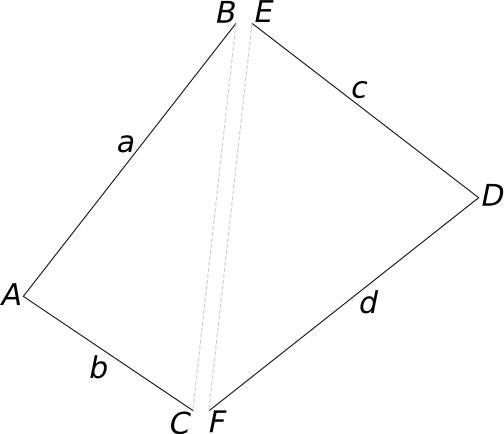
\includegraphics[width=0.7\textwidth]{figura1.png}
   \caption{para que seja possível formar o quadrilátero, as medidas dos segmentos $\overline{BC}$ e $\overline{EF}$ devem ser iguais.}
   \label{fig:formacao-quadrilatero}
  \end{figure}
  
  
  Note a desigualdade acima: ela representa o fato de que estamos lidando com um elemento geométrico (o quadrilátero), cujas medidas são positivas. Dito de outra forma, não adiantará resolvermos a equação acima se, no final, chegarmos à conclusão de que o segmento $\overline{BC}$ (ou $\overline{FE}$) tem medida menor que zero, pois isto não faz sentido. Então, precisamos verificar em que condições essa desigualdade é verdadeira antes de prosseguirmos.
  
  Vejamos o lado esquerdo da equação: como $a$ e $b$ são medidas de um segmento de reta, então certamente $a,b \ge 0$. Neste caso, podemos interpretar os segmentos $\overline{AB}$ e $\overline{AC}$ (de medidas $a$ e $b$, respectivamente) como vetores, e ver no que dá. Assim:
  \begin{equation*}
    a^2 + b^2 - 2ab\cos\hat A = \vec a^2 + \vec b^2 - 2\vec a\vec b = \left(\vec a - \vec b\right)^2 \ge 0.
  \end{equation*}

  Boas notícias: o lado esquerdo da equação \ref{eq:proposicao} é sempre positivo, desde que $a, b \ge 0$, que é o nosso caso. E como o lado direito da mesma equação é isomórfico ao esquerdo (isto é, eles têm a mesma estrutura), podemos estender nossa conclusão para ele. Isto é, se $c, d \ge 0$, então também o lado direito será positivo ou nulo. Desste modo, podemos prosseguir sem qualquer preocupação extra.
  
  Agora, visando utilizar o método dos \emph{multiplicadores de Lagrange}, precisamos reescrever a condição \ref{eq:proposicao} como uma função dos ângulos $\hat A$ e $\hat D$:
  \begin{equation}\label{eq:quadrilatero}
   g(\hat A, \hat D) = (a^2 + b^2) - 2ab\cos\hat A - (c^2 + d^2) + 2cd\cos\hat D = 0.
  \end{equation}
  
  Mas porque $g$ é uma função apenas dos ângulos, já que temos também na expressão as medidas dos lados? A resposta está no enunciado do problema: partimos do pressuposto de que os lados $a$, $b$, $c$ e $d$ são dados e que, com base neles, encontraremos a configuração que maximize a área do quadrilátero. Portanto, os lados são constantes do problema e só podemos variar os ângulos $\hat A$ e $\hat D$. Por outro lado, os ângulos que serão formados ao juntarmos os vértices $B$ com $F$ e $C$ com $E$ (veja a figura) serão definidos quando satisfizermos a equação \ref{eq:proposicao}.
  
  Vamos em frente: a área do quadrilátero pode ser expressa também como uma função de $\hat A$ e $\hat D$, assim:
  \begin{equation}\label{eq:area}
    S(\hat A, \hat D) = \frac{1}{2} ab\sin\hat A + \frac{1}{2}cd\sin \hat D.
  \end{equation}
  
  Assim, o que queremos é maximizar a área \ref{eq:area}, mas isto deve ser feito ao mesmo tempo que satisfazemos \ref{eq:quadrilatero}, pois esta equação é que garante a existência do quadrilátero. Assim, usaremos o multiplicador de Lagrange $\lambda$ e definiremos a expressão
  \begin{equation*}
   L(\hat A, \hat D, \lambda) = S(\hat A, \hat D) - \lambda g(\hat A, \hat D).
  \end{equation*}
  
  $\hat A$ e $\hat D$ devem ser tais que satisfaçam
  \begin{equation*}
   \frac{\partial L}{\partial \hat A} = \frac{\partial L}{\partial \hat D} = \frac{\partial L}{\partial \lambda} = 0
  \end{equation*}
  
  Mas $\partial L/\partial\lambda = g(\hat A, \hat D) = 0$. Portanto, $\hat A$ e $\hat D$ devem satisfazer \ref{eq:quadrilatero} e
  \begin{align}
   \frac{\partial L}{\partial\hat A} &= \frac{1}{2}ab\cos\hat A - 2ab\lambda\sin\hat A = 0 \label{*}\\
   \frac{\partial L}{\partial\hat D} &= \frac{1}{2}cd\cos\hat D - 2cd\lambda\sin\hat D = 0 \label{**}
  \end{align}
  
  De \eqref{*}, $\cos\hat A = 4\lambda\sin\hat A \Rightarrow \tan\hat A = 1/(4\lambda)$; e de \eqref{**}, $\cos\hat D = -4\lambda\sin\hat D \Rightarrow \tan\hat D = -1/(4\lambda)$. Ou seja, $\tan\hat A = -\tan\hat D$, o que significa que
  \begin{equation}\label{eq:D}
   \hat D = \pi - \hat A,
  \end{equation}
  pois $\hat A, \hat D \in [0,\pi]$ e $\tan(\pi - \theta) = -\tan\theta$, para $\theta\in[0,\pi]$.
  
  Levando este resultado a \eqref{eq:proposicao} ou \eqref{eq:quadrilatero} (antes notando que $\cos\hat D = \cos\left(\pi - \hat A\right) = -\cos\hat A$), temos:
  \begin{gather}
   a^2 + b^2 - 2ab\cos\hat A = c^2 + d^2 + 2cd\cos\hat A \Rightarrow\nonumber\\
   \Rightarrow (a^2 + b^2) - 2ab\cos\hat A - (c^2 + d^2) - 2cd\cos\hat A = 0 \Rightarrow\nonumber \\
   \Rightarrow (a^2 + b^2) - (c^2 + d^2) - 2(ab+cd)\cos\hat A = 0 \Rightarrow\nonumber \\
   \Rightarrow \cos\hat A = \frac{(a^2+b^2)-(c^2+d^2)}{2(ab+cd)} \in [-1,1].\label{eq:A}
  \end{gather}

  E como $\cos\hat A$ é uma função unívoca em $[0,\pi]$, $\hat A$ é univocamente determinado quando dados $a$, $b$, $c$ e $d$; e este é sempre solúvel em $\mathbb{R}$ desde que $|\cos\hat A| \le 1$.
  
  Levando agora \eqref{eq:D} em \eqref{eq:area}, podemos encontrar uma forma simplificada para $S(\hat A) \equiv S(\hat A, \hat D(\hat A))$:
  \begin{align*}
   S(\hat A) &= \frac{1}{2}ab\sin\hat A + \frac{1}{2}cd\sin\hat D\\
	     &= \frac{1}{2}ab\sin\hat A + \frac{1}{2}cd\sin\left(\pi - \hat A\right)\\
	     &= \frac{1}{2}ab\sin\hat A + \frac{1}{2}cd\sin\hat A\\
	     &= \frac{1}{2} (ab + cd)\sin\hat A\\
	     &= \frac{1}{2} (ab + cd)\sqrt{1- \cos^2\hat A}.
  \end{align*}
  
  Colocando aí o resultado \eqref{eq:A},
  \begin{align*}
   S(\hat A) &= \frac{1}{2}(ab+cd)\sqrt{1-\frac{\left[(a^2+b^2)-(c^2+d^2)\right]^2}{4(ab+cd)^2}} \\
	     &= \frac{1}{4}\sqrt{4(ab+cd)^2-\left[(a^2+b^2)-(c^2+d^2)\right]^2} \\
	     &= \frac{1}{4}\sqrt{\left\{2(ab+cd)-\left[(a^2+b^2)-(c^2+d^2)\right]^2\right\} \left\{2(ab+cd)+\left[(a^2+b^2)-(c^2+d^2)\right]^2\right\}} \\
	     &= \frac{1}{4}\sqrt{\left(2ab+2cd-a^2-b^2+c^2+d^2\right) \left(2ab+2cd+a^2+b^2-c^2-d^2\right)} \\
	     &= \frac{1}{4}\sqrt{\left[-(a^2-2ab+b^2)+(c^2+2cd+d^2)\right] \left[(a^2+2ab+b^2)-(c^2-2cd+d^2)\right]} \\
	     &= \frac{1}{4}\sqrt{\left[(c+d)^2-(a-b)^2\right] \left[(a+b)^2-(c-d)^2\right]} \\
	     &= \frac{1}{4}\sqrt{(-a+b+c+d)(+a-b+c+d)(a+b-c+d)(a+b+c-d)} \\
	     &= \frac{1}{4}\sqrt{\left[(a+b+c+d)-2a\right] \left[(a+b+c+d)-2b\right] \left[(a+b+c+d)-2c\right] \left[(a+b+c+d)-2d\right]} \\
	     &= \frac{1}{4}\sqrt{2^4\left(\frac{a+b+c+d}{2} - a\right) \left(\frac{a+b+c+d}{2} - b\right) \left(\frac{a+b+c+d}{2} - c\right) \left(\frac{a+b+c+d}{2} - d\right)} \\
	     &= \sqrt{(p-a)(p-b)(p-c)(p-d)},
  \end{align*}
  onde $p=(a+b+c+d)/2$ é o semi-perímetro do quadrilátero. É interessante observar que esta expressão (chamada de fórmula de Brahmagupta), que obtivemos neste caso particular, é bastante genérica, pois ela envolve apenas os lados do quadrilátero. Isto significa que o problema apresentado tem solução única, pois não importa quais foram os lados dados, a área será sempre a mesma, independentemente da forma como os arranjamos.
  
  Uma vez que a quadra $(a,b,c,d)$ forme um quadrilátero (o que equivale a dizer que \eqref{eq:proposicao} ou \eqref{eq:quadrilatero} é satisfeita), $\hat A + \hat B + \hat C + \hat D = 2\pi$. Mas como $\hat A + \hat D = \pi$ (pela equação \ref{eq:D}), é claro que $\hat B + \hat C = \pi$.
  
  Pela lei dos cossenos (novamente. Veja a figura~\ref{fig:cossenos-2}),
  \begin{equation*}
   a^2 + c^2 - 2ac\cos\hat B = b^2 + d^2 - 2bd\cos \hat C.
  \end{equation*}
  
  \begin{figure}
    \centering
   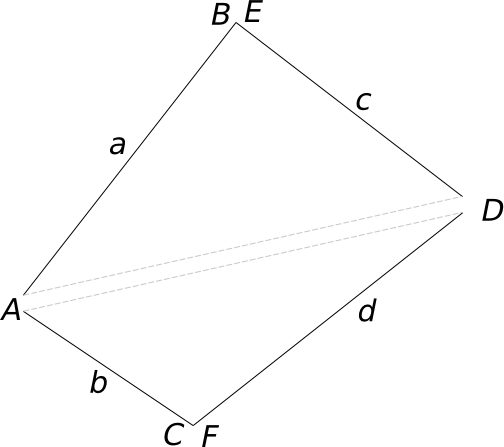
\includegraphics[width=0.7\textwidth]{figura2.png}
   \caption{A lei dos cossenos, de novo.}
   \label{fig:cossenos-2}
  \end{figure}
  
  Note que agora não precisamos impor nenhuma condição extra. E como $\hat C = pi - \hat B$, $\cos \hat C = -\cos \hat B$. Logo,
  \begin{equation}
   \cos \hat B = \frac{(a^2 + c^2) - (b^2 + d^2)}{2(ac + bd)} \in [-1,1].
  \end{equation}
  
  Resumindo: dados quatro lados $a$, $b$, $c$ e $d$ que formem um quadrilátero, sempre haverá um quadrilátero formado por esses lados cuja área é máxima e independente da organização desses lados: $S = \sqrt{(p-a)(p-b)(p-c)(p-d)}$. Ou seja, esse quadrilátero é único. Para formá-lo, precisaremos conhecer os ângulos:
  \begin{align*}
   \cos\hat A &= \frac{a^2+b^2-c^2-d^2}{2(ab+cd)} \\
   \cos\hat B &= \frac{a^2-b^2+c^2-d^2}{2(ac + bd)} \\
       \hat C &= \pi - \hat B \\
       \hat D &= \pi - \hat A.
  \end{align*}

  \paragraph{Comentários:} é interessante observar que partimos do problema de maximizar a área do quadrilátero, que em princípio poderia variar conforme a configuração dos lados. Porém, se tivéssemos observado, desde o início, a fórmula de Brahmagupta, chegaríamos à conclusão de que, uma vez formado o quadrilátero, sua áre é independente do arranjo dos lados. Portanto, a (única) área possível é a área máxima, dada por esta fórmula. A condição de formação do quadrilátero também tem uma forma mais fácil e conhecida que a que usamos: a medida de um lado qualquer deve ser menor ou igual à soma dos demais lados.
  
  Curiosamente, o multiplicador de Lagrange só foi útil para encontrar a expressão $\hat D = \pi - \hat A$. Com essa igualdade formamos um sistema de quatro equações e quatro incógnitas, usando as duas leis dos cossenos e a soma dos ângulos internos.







  

  
  
  

\end{document}
